\section{Experimento BRDF Dür}

No artigo de Geisler-Moroder e Dür \cite{duer2010bounding}, são discutidas as limitações do modelo de reflexão de Ward, propondo uma abordagem para restringir o albedo e garantir a conservação de energia. Este experimento é baseado nessa BRDF com albedo restringido. As equações são apresentadas na \autoref{fig-duer-eqlang-latex}, com o código fonte em \texttt{EquationLang} disponível no \autoref{cod-duer-eqlang}. Os códigos gerados em GLSL podem ser vistos no \autoref{cod-duer-glsl-pt-1} e no \autoref{cod-duer-glsl-pt-2}. A renderização dos objetos 3D pode ser observada na \autoref{fig-duer-eqlang} e os \textit{plots} na \autoref{fig-duer-plots}.

%%%%%%%%%%%%%%%%%%%%%%%%%%%%%%%%%%%%%%%%%%%%%%%%%
\subsection{Representação em documento \LaTeX{}}
%%%%%%%%%%%%%%%%%%%%%%%%%%%%%%%%%%%%%%%%%%%%%%%%%
\begin{figure}[H]
    \caption{\label{fig-duer-eqlang-latex} \small Equações da BRDF do experimento duer em documento \LaTeX{}.}
    \begin{center}
        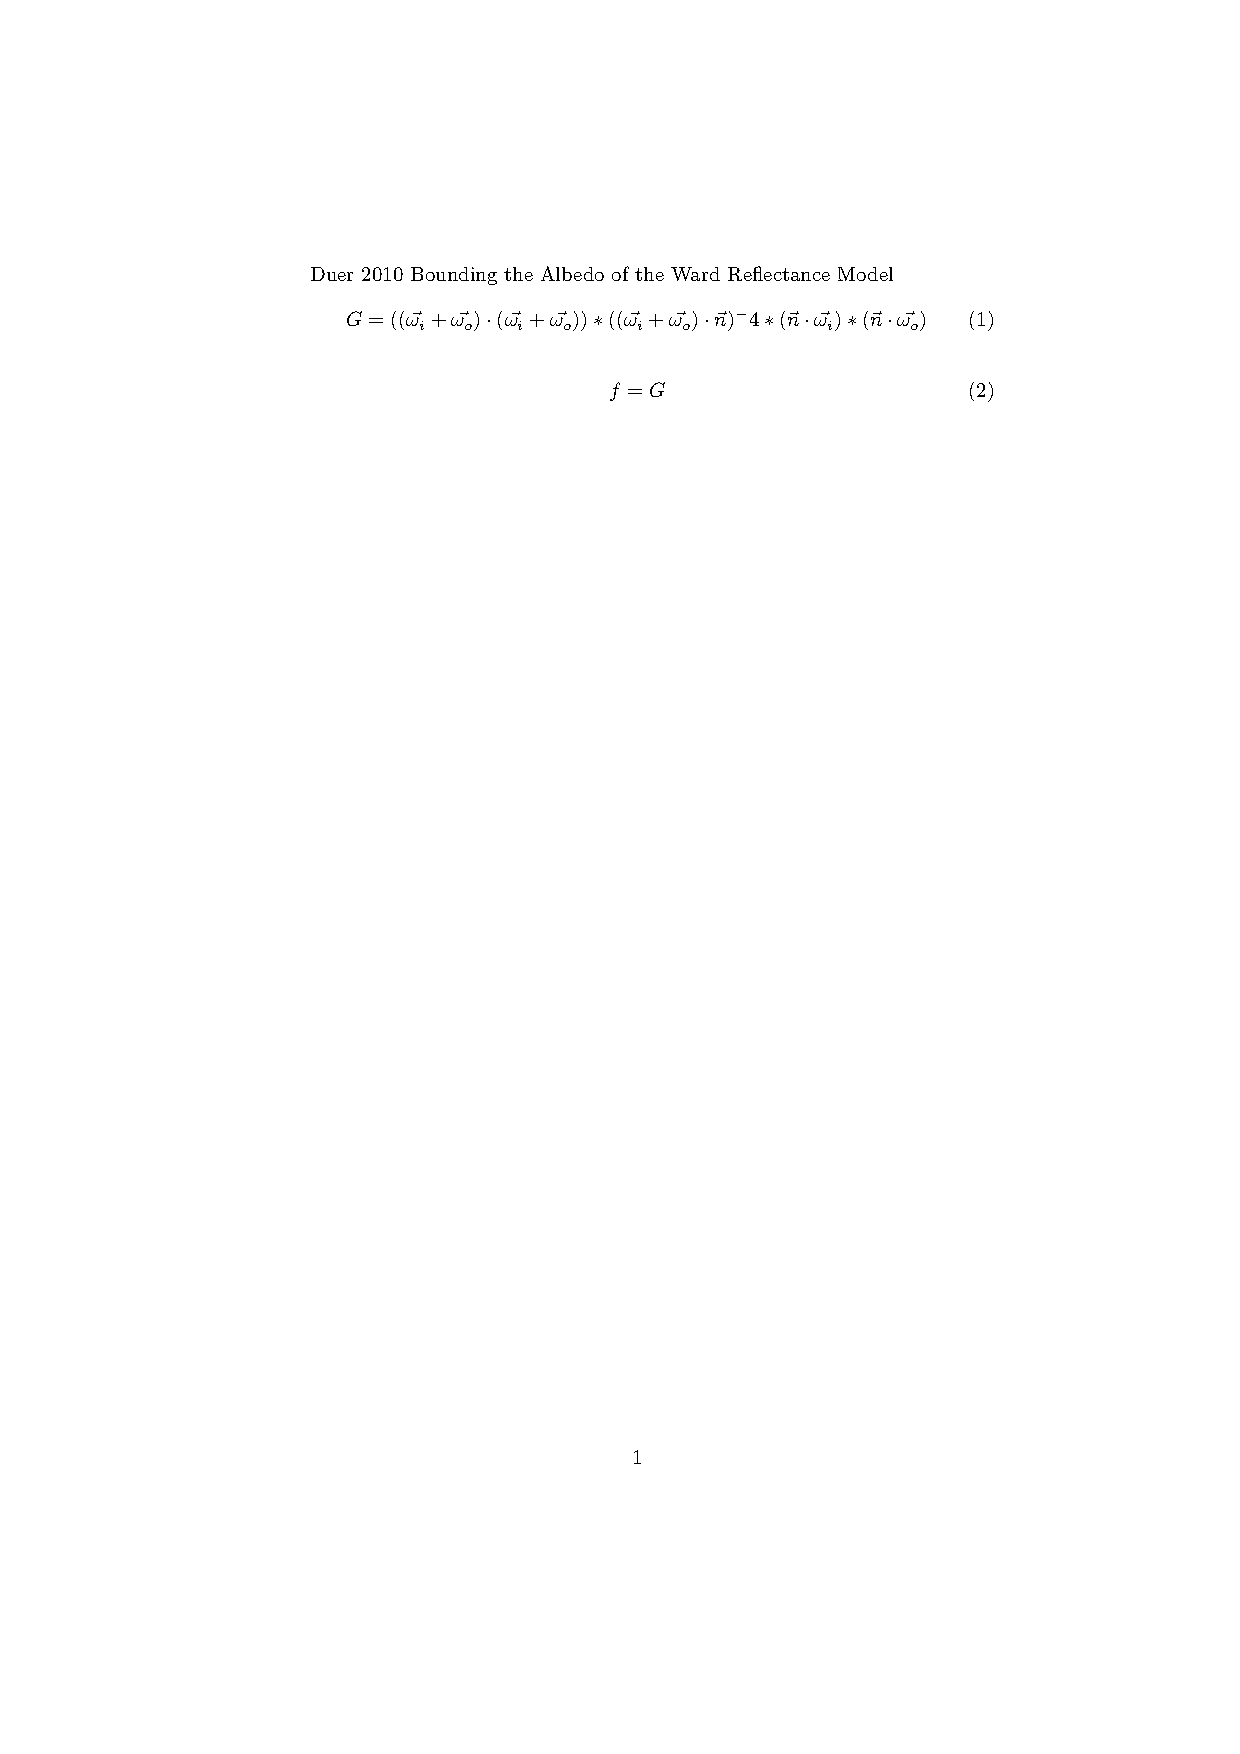
\includegraphics[scale=0.92]{./Imagens/brdfs/duer.pdf}
    \end{center}
\end{figure}

%%%%%%%%%%%%%%%%%%%%%%%%%%%%%%%%%%%%%%%%%%%%%%%%%
\subsection{Código Fonte em \texttt{EquationLang}}
%%%%%%%%%%%%%%%%%%%%%%%%%%%%%%%%%%%%%%%%%%%%%%%%%
\begin{codigo}[H]
    \caption{\small Código fonte da BRDF deste experimento.}
    \label{cod-duer-eqlang}
\begin{lstlisting}[language=tex, frame=none, inputencoding=utf8]
Duer 2010 Bounding the Albedo of the Ward Reflectance Model

\begin{equation}
G = ((\vec{\omega_i}+\vec{\omega_o}) \cdot(\vec{\omega_i}+\vec{\omega_o})) * ((\vec{\omega_i}+\vec{\omega_o}) \cdot \vec{n})^-4
    * (\vec{n} \cdot \vec{\omega_i})*(\vec{n} \cdot \vec{\omega_o})
\end{equation}

\begin{equation}
f =  G
\end{equation}
\end{lstlisting}
\end{codigo}

%%%%%%%%%%%%%%%%%%%%%%%%%%%%%%%%%%%%%%%%%%%%%%%%%
\subsection{Código GLSL Gerado}
%%%%%%%%%%%%%%%%%%%%%%%%%%%%%%%%%%%%%%%%%%%%%%%%%
\begin{codigo}[H]
    \caption{\small Saída do compilador: código GLSL da BRDF deste experimento (parte 1 de 2).}
    \label{cod-duer-glsl-pt-1}
\begin{lstlisting}[language=C, inputencoding=utf8]
analytic ::begin parameters
#[type][name][min val][max val][default val]
::end parameters
::begin shader
//////////// START OF BUILTINS DECLARTION ////////////
vec3 var_0_vec_h;
vec3 var_3_vec_n;
float var_10_theta_h;
float var_11_theta_d;
float var_1_pi;
float var_2_epsilon;
vec3 var_4_vec_omega_i;
float var_5_theta_i;
float var_6_phi_i;
vec3 var_7_vec_omega_o;
float var_8_theta_o;
float var_9_phi_o;
//////////// END OF BUILTINS DECLARTION ////////////
//////////// START OF USER DECLARED ////////////
float var_12_G;
float var_13_f;
//////////// END OF USER DECLARED ////////////
//////////// START FUNCTIONS DECLARATIONS ////////////
//////////// END FUNCTIONS DECLARATIONS ////////////

\end{lstlisting}
\end{codigo}

\begin{codigo}[H]
    \caption{\small Saída do compilador: código GLSL da BRDF deste experimento (parte 2 de 2).}
    \label{cod-duer-glsl-pt-2}
\begin{lstlisting}[language=C, inputencoding=utf8]
vec3 BRDF(vec3 L, vec3 V, vec3 N, vec3 X, vec3 Y) {

  //////////// START OF BUILTINS INITIALIZATION ////////////
  var_0_vec_h = normalize(L + V);
  var_3_vec_n = normalize(N);
  var_1_pi = 3.141592653589793;
  var_2_epsilon = 1.192092896e-07;
  var_4_vec_omega_i = L;
  var_5_theta_i = atan(var_4_vec_omega_i.y, var_4_vec_omega_i.x);
  var_6_phi_i = atan(sqrt(var_4_vec_omega_i.y * var_4_vec_omega_i.y +
                          var_4_vec_omega_i.x * var_4_vec_omega_i.x),
                     var_4_vec_omega_i.z);
  var_7_vec_omega_o = V;
  var_8_theta_o = atan(var_7_vec_omega_o.y, var_7_vec_omega_o.x);
  var_9_phi_o = atan(sqrt(var_7_vec_omega_o.y * var_7_vec_omega_o.y +
                          var_7_vec_omega_o.x * var_7_vec_omega_o.x),
                     var_7_vec_omega_o.z);
  var_10_theta_h = acos(dot(var_0_vec_h, N));
  var_11_theta_d = acos(dot(var_0_vec_h, var_4_vec_omega_i));
  //////////// END OF BUILTINS INITIALIZATION ////////////

  var_12_G =
      ((((dot(((var_4_vec_omega_i + var_7_vec_omega_o)),
              ((var_4_vec_omega_i + var_7_vec_omega_o)))) *
         pow((dot(((var_4_vec_omega_i + var_7_vec_omega_o)), var_3_vec_n)),
             (-4.0))) *
        (dot(var_3_vec_n, var_4_vec_omega_i))) *
       (dot(var_3_vec_n, var_7_vec_omega_o)));
  var_13_f = var_12_G;

  return vec3(var_13_f);
}
\end{lstlisting}
\end{codigo}


%%%%%%%%%%%%%%%%%%%%%%%%%%%%%%%%%%%%%%%%%%%%%%%%%
\subsection{Visualização do Resultado}
%%%%%%%%%%%%%%%%%%%%%%%%%%%%%%%%%%%%%%%%%%%%%%%%%
\begin{figure}[H]
    \caption{\small{\textit{Plots} da distribuição de reflexão especular e difusa deste experimento.}}
    \label{fig-duer-plots}
\minipage{0.48\textwidth}
    \vspace{42px}
  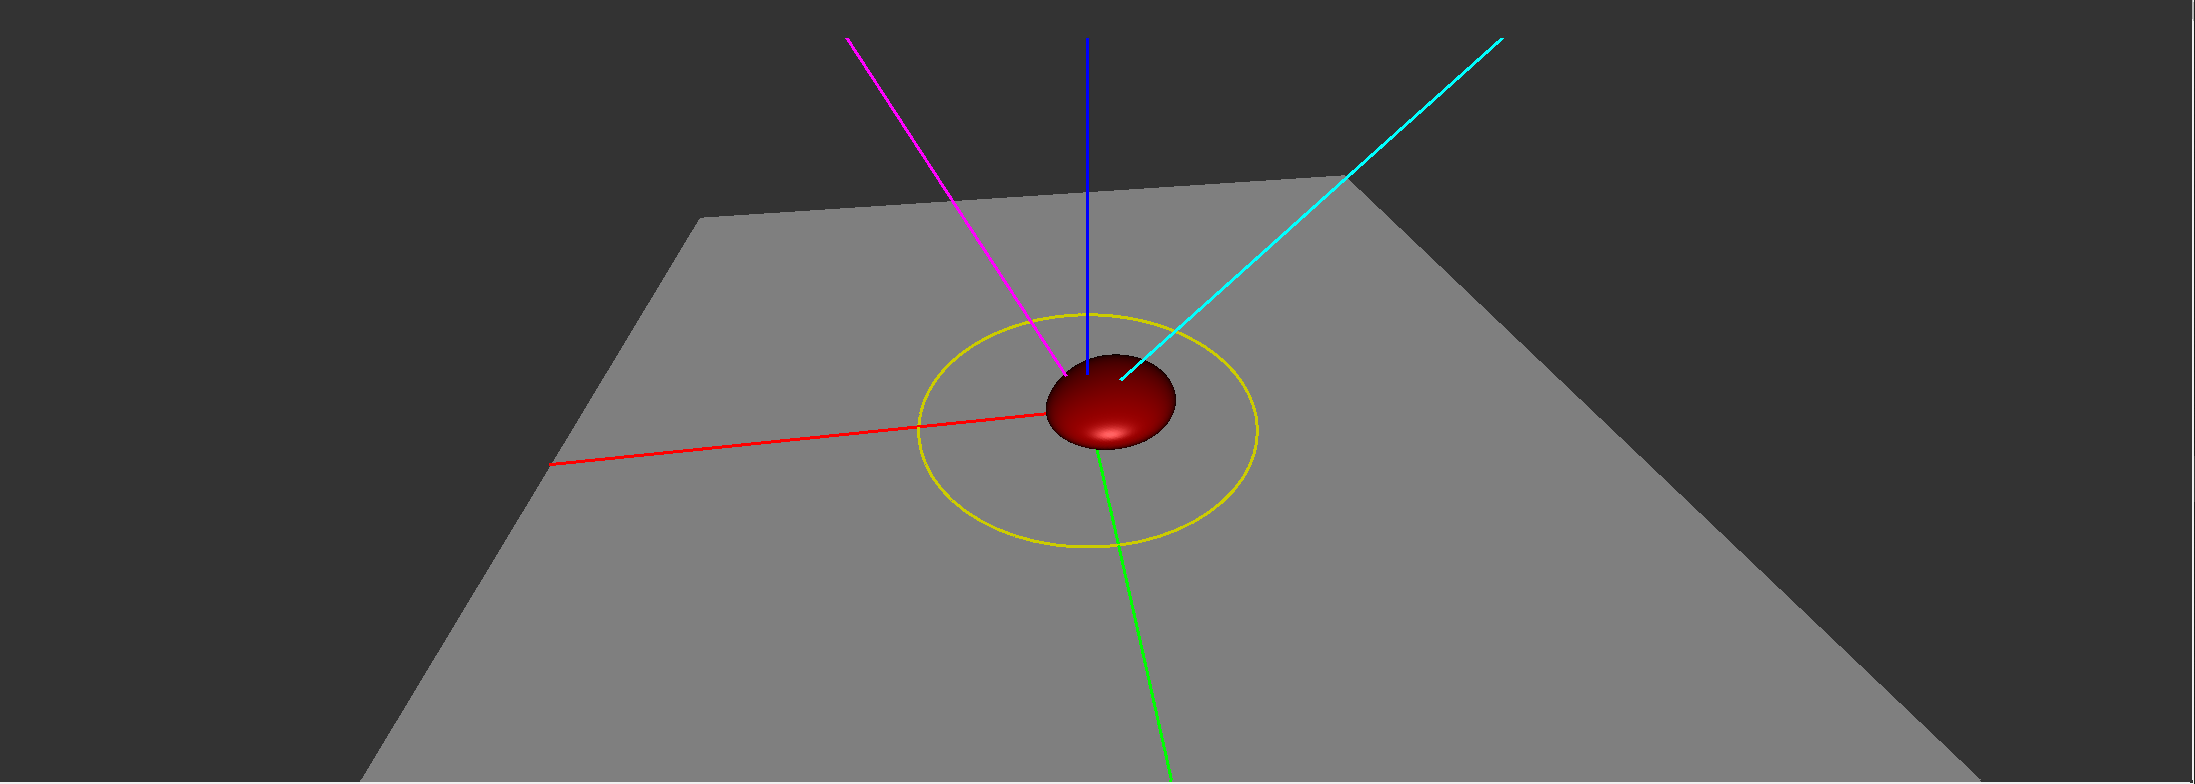
\includegraphics[width=\linewidth]{./Imagens/brdfs/duer-3D-plot}
    % \vspace{0.1px}
    \legend{ \small (a) 3D \textit{plot}}
\endminipage\hfill
\minipage{0.48\textwidth}
  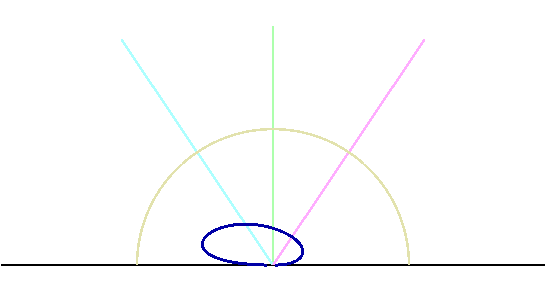
\includegraphics[width=\linewidth]{./Imagens/brdfs/duer-polar-plot.png}
    \legend{ \small (b) \textit{Polar plot}}
\endminipage\hfill
\end{figure}

\begin{figure}[H]
    \caption{\small{Objetos 3D renderizados por este experimento.}}
    \label{fig-duer-eqlang}
\minipage{0.32\textwidth}
  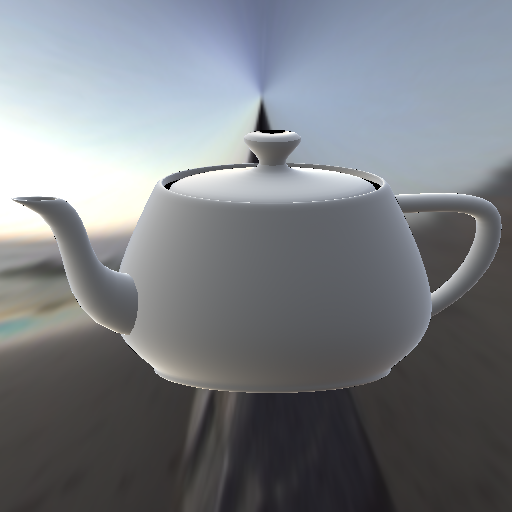
\includegraphics[width=\linewidth]{./Imagens/brdfs/duer-teapot.png}
    \legend{ \small (a) \textit{Teapot}}
\endminipage\hfill
\minipage{0.32\textwidth}
  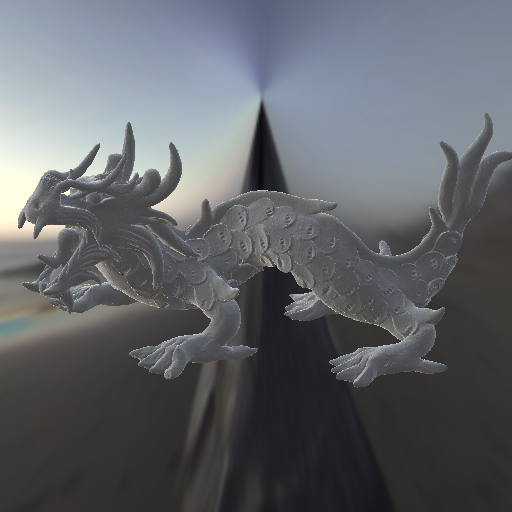
\includegraphics[width=\linewidth]{./Imagens/brdfs/duer-dragon.png}
    \legend{ \small (b) Dragão de Stanford}
\endminipage\hfill
\minipage{0.32\textwidth}%
  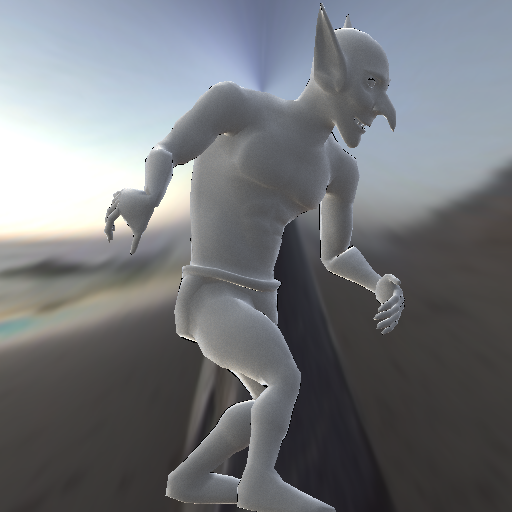
\includegraphics[width=\linewidth]{./Imagens/brdfs/duer-goblin.png}
    \legend{ \small (c) Goblin}
\endminipage
\end{figure}

